\documentclass[12pt,a4paper]{article}

\usepackage{amsmath,amsthm,amssymb}
\usepackage[utf8]{vietnam}
\usepackage{blindtext}
\usepackage{listings}
\usepackage{graphicx}
\usepackage[numbers]{natbib}
\usepackage{enumitem}
\renewcommand{\baselinestretch}{1.5}
\begin{document}

%----------------------------------------------------------------------------------------
%	TITLE PAGE
%----------------------------------------------------------------------------------------

\begin{titlepage} % Suppresses displaying the page number on the title page and the subsequent page counts as page 1
	\newcommand{\HRule}{\rule{\linewidth}{0.5mm}} % Defines a new command for horizontal lines, change thickness here
	
	\center % Centre everything on the page
	
	%------------------------------------------------
	%	Headings
	%------------------------------------------------
	
	\textsc{\LARGE đại học khoa học tự nhiên}\\[1.5cm] 
	\textsc{\Large Khoa Toán-tin học}\\[0.5cm] 
	
	\textsc{\large Phương pháp toán trong tin}\\[0.5cm] 
	
	%------------------------------------------------
	%	Title
	%------------------------------------------------
	
	\HRule\\[0.4cm]
	
	{\huge\bfseries The World's Hardest Game với Phương pháp học tăng cường}\\[0.4cm] % Title of your document
	
	\HRule\\[1.5cm]
	
	%------------------------------------------------
	%	Author(s)
	%------------------------------------------------
	
	\begin{minipage}{0.4\textwidth}
		\begin{flushleft}
			\large
			\textit{Tác giả}\\
			\textsc{Phan Quang Khánh} % Your name
		\end{flushleft}
	\end{minipage}
	~
	\begin{minipage}{0.4\textwidth}
		\begin{flushright}
			\large
			\textit{Giảng viên hướng dẫn}\\
			TS. Huỳnh Thế \textsc{Đăng} % Supervisor's name
		\end{flushright}
	\end{minipage}
	
	\vfill\vfill\vfill % Position the date 3/4 down the remaining page
	
	{\large\today} % Date, change the \today to a set date if you want to be precise
	
	%------------------------------------------------
	%	Logo
	%------------------------------------------------
	
	%\vfill\vfill
	%\includegraphics[width=0.2\textwidth]{placeholder.jpg}\\[1cm] % Include a department/university logo - this will require the graphicx package
	 
	%----------------------------------------------------------------------------------------
	
	\vfill % Push the date up 1/4 of the remaining page
	
\end{titlepage}
%---------------------------------------------------------------------------------
\clearpage
\tableofcontents
\clearpage
\noindent \section{Đặt vấn đề}\\
The World’s Hardest Game là một trò chơi trực tuyến nổi tiếng trong năm 2015 với cách chơi khó nhưng đủ khiến kích thích người chơi cố gắng vượt qua bởi tưởng “dễ nhưng không dễ” của nó. Trong trò chơi, người chơi có thể di chuyển bằng 4 hướng (trên, dưới, trái, phải) với mục đích hoàn thành cách thức chơi của mỗi vòng. Để hoàn thành một vòng chơi, người chơi phải thu thập hết các đồng xu, tránh va phải các kẻ thù và di chuyển đến vùng qua màn. Vì trò chơi là tất định? Nó rất khó để con người có thể hoàn thành, cần biết trước được có gì, kiên nhẫn và chiến thuật “kì dị”. Tuy nhiên, tập các hành động có thể thực hiện ở bất cứ thời gian nào là hữu hạn và phần thưởng cho một hành động rất dễ dàng để tính. Do đó TWHG là một ứng cử viên tốt cho một mô hình học tăng cường \footnote{reinforcement learning model}.\\
\\
Mục định chính của đề tài là sử dụng Deep Q-learning với Experience Replay được sử dụng bởi DeepMind để huấn luyện một mô hình có thể đánh bại TWHG, vượt qua khả năng chơi của con người.
\clearpage
\section{Cơ sở lý thuyết}\\
\subsection{Học tăng cường}
Q-learning, trong đó đối tượng trong trò chơi\footnote{agent} tối ưu hàm phần thưởng đặc trưng của trò chơi bằng việc chọn hành động để tối đa hóa hàm tích lũy phần thưởng trong tương lai, là một trong những kỹ thuật mô hình hóa môi trường của agent và tập hành động của nó bằng quá trình quyết định Markov hữu hạn\footnote{finite Markov decision process}.\\
\subsection{Học tăng cường chuyên sâu}
Lợi thế trong học sâu\footnote{Deep learnning} cũng mang lại lợi thế cho Deep Q-learning, việc tìm kiếm trên bảng Q -value có thể được ước lượng bằng mạng thần kinh\footnote{nerual net} dẫn đến có thể tìm hàm Q trong không gian lớn hơn và tập action rộng hơn mà không cần phải mở rộng ra hết mọi khả năng có thể của trò chơi (đơn giản hóa). Ngoài ra, lớp tích chập\footnote{convolutional layer} cho phép mô hình có thể học trực tiếp từ những khung hình của trò chơi.
\subsection{Mô phỏng trò chơi}
Nhóm tác giả sử dụng flash bằng việc sử dụng thư viện selenium để thực hiện các hành động trên các trình duyệt.
\begin{figure}[h]
    \centering
    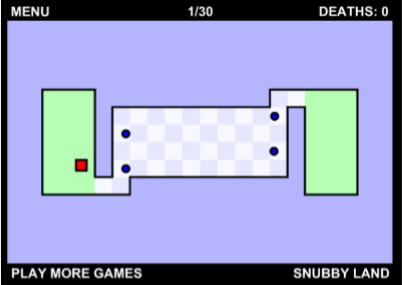
\includegraphics{photo/lv1game.png}
    \caption{Vòng đầu tiên của TWHG}
    \label{fig:my_label}
\end{figure}
\section{Hướng tiếp cận}
Hướng tiếp cận dựa trên bài báo cáo của một nhóm cựu học sinh trường MIT. Sau vài tuần huấn luyện, mục tiêu của bài này nằm ngoài kiến thức của tác giả, với mô hình tốt nhất cũng chỉ cố gắng thoát khỏi vùng bắt đầu của trò chơi. Do đó, tác giả mở rộng một vài “toy” games, thử bằng các kỹ thuật và siêu tham số\footnote{hyperparameters} của DeepMind để đánh bại 2 mô hình: mô hình ngẫu nhiên\footnote{random model} và  mô hình  $\epsilon$.\\
\subsection{Toy games}
Như đã được trình bày ở trong phần giới thiệu, không thể huấn luyện mô hình trực tiếp từ mô phỏng của chính trò chơi. Do đó nhóm tác giả cho ra ba trò chơi nhỏ hơn nhằm mô phỏng lại trò chơi.
\subsubsection{Toy Game 1-D (TG1D)}
Trò chơi đầu tiên rất đơn giản, bao gồm 1 mảng 1 chiều  với 4 ô với sự xuất hiện ngẫu nhiên của kẻ thù ở 1 trong 4 ô. Kẻ thù $e$ có thể xuất hiện và biến mất trong một giai đoạn và nhiệm vụ của người chơi $p$ là di chuyển từ ô thứ nhất sang ô thứ 4 mà không xuất hiện cùng lúc với kẻ thủ ở cùng một vị trí. Tập hành động có thể có của $p$ là \{trái, phải, dừng\}. Định nghĩa về một vector trạng thái như sau:\\
\begin{align*}
S_x=\begin{cases}
-2\quad \quad &\text{khi $e=x$ và $p=x$}\\
-1\quad \quad &\text{khi $e=x$}\\
1 \quad \quad &\text{khi $p=x$}\\
0 \quad \quad &\text{trường hợp còn lại}
\end{cases}
\end{align*}
\subsubsection{Toy Game 2-D (TG2D)}
Trò chơi được chơi trên một vùng gồm 4x4 ô vuông, và $p$ được bắt đầu ở vị trí (0,0) và kết tại vị trí (3,3). Bên cạnh đó sẽ có duy nhất một $e$ xuất hiện ngẫu nhiên tại các ô tuy nhiên $e$ không xuất hiện ở ô bắt đầu và ô kết thúc trong một khoảng thời gian ngẫu nhiên. Cũng tương tự như cách chơi của TG1D nhưng $p$ được di chuyển trên tập lớn hơn \{lên, xuống, trái, phải, dừng\}. Xây dựng vector trạng thái tương tự như TG1D khi làm dẹp không gian 2D thành 1D.
\subsubsection{Toy Game 2-D - Hard (TG2D-H)}
Trò chơi được xây dựng giống như TG2D thay vì chỉ có một $e$ thì bây giờ sẽ có nhiều hơn.
\begin{figure}[t]
    \centering
    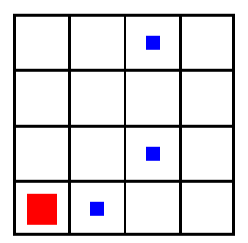
\includegraphics{photo/TG2D_H.png}
    \caption{TG2D-H}
    \label{fig:my_label}
\end{figure}
\subsection{Learning}
Thực hiện mạng nơ-ron\footnote{neural model} cho mô hình này, nhóm tác giả sử dụng thư viện Tensorflow. Đầu ra của mạng\footnote{net} được lấy từ kết quả của Q-dự đoán\footnote{Q-estimate} cho mỗi hành động, với hành động tốt nhất được định nghĩa là $\arg \max_{a \in \mathcal{A}} Q(t,a)$. Hàm mục tiêu\footnote{Loss function} được dùng để tối ưu là Sai số bình phương trung bình\cite{mse} giữa Q-dự đoán được dự đoán từ  hành động $a$ tại thời điểm $t$ cho trước và "nhận ra" Q-giá trị \footnote{"realised" Q-value}, được xem là phần thưởng đã biết cho $a$ tại $t$ cộng với discount Q-dự đoán của hành động tốt nhất tại thời điểm $t+1$, biết $a$ và $t$. Dưới đây là công thức tính hàm mất mất của từng minibatch $\mathcal{B}$, lấy mẫu từ replay memory $\mathcal{M}$.\\
\[\mathcal{L} = \dfrac{1}{|\mathcal{B}|}\sum_{t\in \mathcal{B}}\left[\left(Q(t,a_t) - \left[r_{t,a} + \gamma \max_{a\in \mathcal{A}} Q(t+1,a)\right]\right)\right]^2\]
Các mẫu được tạo ra từ kỹ thuật Experience Replay được mô tả từ bài báo DeepMind, với một quy luật $\epsilon$-tham lam\footnote{$\epsilon$-greedy policy} cho việc chọn hành động tối ưu (với $\epsilon$ điều khiển lúc nào hành động ngẫu nhiên được thực thi, để bắt buộc việc mở rộng hành động\footnote{exploration}). Replay memory của từng tập\footnote{episode} được bắt đầu tạo bởi việc làm đầy các lịch sử $\mathcal{H}$ với $|\mathcal{H}|$ là số khung hình của người chơi thực hiện động tác \texttt{dừng}. Điều này là một đặc tính khá tốt để mô hình có thể nhận dạng được bước đi của kẻ thù để bắt đầu di chuyển.\\
Cấu trúc của mô hình được xây dựng như cấu trúc trong bài báo DeepMind\cite{deepmindpaper}, với đầu vào là hình ảnh của từng khung hình và số lượng 3 hoặc 5 node đầu ra, dựa trên trò chơi. Mô hình sử dụng mạng nơ-ron gồm 2 lớp ẩn được kết nối đầy đủ \footnote{fully connected hidden layers} cho đầu vào là một vector trạng thái lần lượt có 128 và 64 ReLU node.\\
\begin{figure}[t]
    \centering
    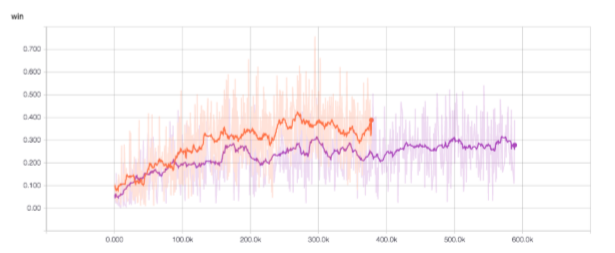
\includegraphics{photo/2model.png}
    \caption{Tỉ lệ thắng trong việc huấn luyến TG2D-H}
    \label{fig:my_label}
\end{figure}
Kết quả cho ra được như Hình 3 với màu cam là mô hình [128,64] và màu tím là mô hình [256,256]\\
\subsection{Siêu tham số}
Hầu hết các siêu tham số trong hệ thống cũng được lấy từ bài báo DeepMind, sau đó điều chỉnh hợp lý hơn cho tập các trò chơi (toy games). \\
\\
Giá trị $\gamma$ ban đầu được dùng là $0.90$, điều này hiệu quả trong việc "phạt" các phần thưởng tương lai để không khuyến khích người chơi từ việc bị "mắc kẹt", điều này thường xảy ra khi toàn bộ hành động \texttt{không phải là dừng} có Q-giá trị âm (thường gần điểm bắt đầu của một phiên huấn luyện). Thử nghiệm với giá trị $0.99$ với hi vọng là giá trị phần thưởng tương lai có thể làm người chơi e dè hơn. Thật vật, với kết quả có được khiến cho người chơi \textttd{dừng} vô cùng tận.\\
\\
$\epsilon$, là tham số quyết định xem một hành động ngẫu nhiên được thực thi khi mô hình mở rộng môi trường, bắt đầu từ 0.9 và giảm tuyến tính xuống còn 0.1, sau $10^5$ khung hình.\\
\\
Minibatch được dùng có kích thước 32. Vì thời gian có hạn nên không thể lấy được kích thước như mô hình của DeepMind là $10^6$, do đó minibatch được tạo mẫu từ replay memory với kích thước $10^5$ với mong muốn là sự thay đổi về kích thước không ảnh hưởng đến kết quả cuối cùng. Kết quả mang lại là thời gian huấn luyện và năng suất tăng rõ rệt.\\
\\
Có thể thấy có 2 cách để xây dựng mô hình để giải quyết bài toán: sử dụng CNN để lấy thông tin rồi quyết định hành động cho trạng thái hoặc phân tách thành các vector trạng thái  và sử dụng mô hình FC. Sau kết quả trên của ta có thể thấy CNN cho ít thông tin hơn nên phần kết quả là sử dụng mô hình FC để giải quyết bài toán.
\subsection{Kết quả}
Nhóm tác giả sử dụng 2 mô hình trên cho cả 3 toy game. Nhưng thời gian huấn luyện bị hạn chế, và việc sử dụng flash khó khăn hơn việc tạo ra một toy games. Do đó sau hơn 1 tuần huấn luyện, nhóm tác giả không có kết quả tốt để báo cáo.\\
Kết quả sau là được chạy 10 lượt, mỗi lượt chứa 1000 games, tất cả có 10,000 mẫu.
\begin{enumerate}[label=\Alph*.]
\item \textit{Random}: Thực hiện mô hình ngẫu nhiên là mô hình chính. Mô hình tạo mẫu của hành động theo phân phối chuẩn
\begin{figure}[h!]
    \centering
    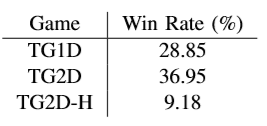
\includegraphics{photo/result1.png}
\end{figure}
\item \textit{$\epsilon$-Greedy}: Mô hình thứ 2 tạo mẫu hành động theo phân phối chuẩn với xác suất tạo là $\epsilon$ và chọn hành động tham lam tại $t+1$ dựa trên phần thưởng tại $t$ với xác suất $1-\epsilon$. Cụ thể sử dụng $\epsilon=0.05$
\\
\\
\begin{figure}[h]
    \centering
    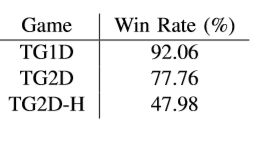
\includegraphics{photo/result2.png}
\end{figure}
\end{enumerate}
\\
\\
\section{Cơ hội và định hướng}
Dựa trên các phương pháp giải quyết của bài báo cáo\cite{report}, ta có thấy nhóm tác giả chỉ thực hiện để tài trong 1 tháng nên có rất nhiều thứ có thể cải thiện.
\subsection{Cơ hội}
\subsubsection{Mô phỏng trò chơi}
Nhóm tác giả sử dụng flash và trình duyệt để mô phỏng trò chơi làm cho thời gian huấn luyện mất nhiều thời gian hơn. Và sắp tới các trình duyệt cùng lúc bỏ flash nên việc thực hiện lại trên ý tưởng này là rất khó. Và nhóm tác giả không thể đưa ra được biễu diễn trực quan trên flash.\\
Lí do trò chơi không có mô phỏng bằng ngôn ngữ Python khiến cho việc huấn luyện dữ liệu cũng như can thiệp vào trò chơi là không có (tốc độ điều khiển, tốc độ kẻ thù,vị trí chướng ngại vật, vị trí phần thưởng thêm,\dots). Do đó việc phân tích và chỉnh sửa mã nguồn Java của trò chơi là tiềm năng cần được khai thác.
\subsubsection{Thời gian thực hiện}
Thời gian thực hiện của nhóm tác giả chưa đủ để có một bản báo cáo tốt như được trình bày ở trên. Do đó sự chuẩn bị trước cho luận văn tốt nghiệp giúp cho thời gian thực hiện đề tài hợp lý hơn.
\clearpage
\subsection{Định hướng}
\textit{Mô phỏng trò chơi:} 
\begin{itemize}
    \item Nhóm đang can thiệp vào mã nguồn java của TWHG với mục đích tạo nhiều hơn một đối tượng để tìm kiếm phương án tốt hơn.
    \item Thay vì huấn luyện từng toy games theo cách ngãu nhiên, nhóm cố trích xuất không gian trò chơi và tạo thành các state vector để huấn luyện trực tiếp.
    \item Tùy biến các tham số cùng thay đổi vận tốc của chương trình để giúp việc huấn luyện nhanh hơn.
    \item Cố gắng tạo ra API có thể biểu diễn được chương trình.
\end{itemize} \\
\textit{Toy games:} Có thể thấy kết quả của TG2D-H vẫn còn thấp nên việc tìm kiếm phương án biểu diễn tốt hơn. Ngoài ra, nhóm cho giả thiết rằng TG1D có thể đạt được kết quả tốt nhất nếu có thời gian huấn luyện nhiều hơn.\\
\\
\textit{Thiết bị huấn luyện:} Nhóm sẽ cố gắng tìm kiếm sự giúp đỡ của bộ môn hoặc thuê các máy chủ ảo để huấn luyện (Google Cloud, AWS, \dots).\\
\\
\textit{Siêu tham số:} Cũng dựa trên hệ thống của DeepMind và sau đó điều chỉnh phù hợp với mô hình được hoàn thiện của nhóm. Phần này được điều chỉnh sau cùng.\\
\clearpage
\addcontentsline{toc}{section}{Tài liệu}
\begin{thebibliography}{9}
\bibitem{deepmindpaper} 
Volodymyr Mnih et al. “Playing Atari with Deep Reinforcement Learning”. In: CoRR abs/1312.5602 (2013).
\\\texttt{http://arxiv.org/abs/1312.5602}

\bibitem{report} 
MIT 6.867: Reinforcement Learning to beat The World's Hardest Game 
\\\texttt{https://github.com/yasyf/hardest-game/blob/master/tex/report/report.pdf}
\end{thebibliography}
\end{document}
